\section{Problem 1: VAE Synthetic Data with Low-Data Stabilization}

\subsection{Objective}
The objective of this problem is to train a Conditional Variational Autoencoder (VAE) using a limited dataset of only 350 real examples per digit, and to evaluate the effectiveness of generating synthetic samples for low-data stabilization. 

\subsection{Methodology}
\begin{enumerate}
    \item \textbf{Augmentation:} The 350 real examples per digit were first augmented by 10-20 times using rotations, shifts, small scaling, and light noise.
    \item \textbf{Training the VAE:} A conditional VAE was trained on the combination of real and augmented data.
    \item \textbf{Generation:} We sampled latent vectors $z \sim \mathcal{N}(0,I)$ to generate $5\times$ synthetic samples per digit (50,000 images in total).
    \item \textbf{Confidence Filtering:} A LeNet-5 model, trained only on the 350 real examples, acted as a "Judge." The generated samples were passed through this classifier, and the maximum softmax output was taken as the confidence level.
\end{enumerate}

Based on the confidence levels, three datasets were created:
\begin{itemize}
    \item \textbf{Set A:} All generated samples.
    \item \textbf{Set B:} High-confidence samples (Confidence $\geq 0.9$).
    \item \textbf{Set C:} Mid-confidence samples ($0.6 \leq \text{Confidence} \leq 0.9$).
\end{itemize}

\subsection{Results \& Conclusion}
A new LeNet-5 was trained using the 350 real examples plus the selected VAE-generated samples for each set. The performance was then compared against the 350-real and 1000-real baselines.

\textit{Question: Does VAE-generated data benefit more from high-confidence selection or mid-confidence/diverse latent samples, and how does it compare with GAN-generated data and simple augmentation?}

\textbf{Answer:} 
\begin{itemize}
    \item VAE-generated data benefits significantly from \textbf{high-confidence selection (Set B)}. High confidence data ($\geq 0.9$) acts as clean, high-quality reinforcement, preventing the model from learning blurry or confused VAE artifacts.
    \item Yes, it successfully reduces the need for real data. The VAE-augmented dataset (97.75\%) successfully matched or outperformed the pure 1000-Real dataset (97.50\%). This proves generative models can effectively synthesize missing data.
\end{itemize}

\vspace{1em}
\begin{table}[h!]
\centering
\begin{tabular}{|l|l|c|c|c|}
\hline
\textbf{Model} & \textbf{Metric} & \textbf{All Gen Data (Set A)} & \textbf{CL $\geq$ 0.9 (Set B)} & \textbf{0.6 $\leq$ CL $\leq$ 0.9 (Set C)} \\ \hline
\multirow{2}{*}{VAE} & No. of Examples & 50000 & 31289 & 12298 \\ \cline{2-5}
                     & Test Accuracy   & 97.60\% & 97.75\% & 96.90\% \\ \hline
\multirow{2}{*}{GAN} & No. of Examples & 50000 & 27252 & 14803 \\ \cline{2-5}
                     & Test Accuracy   & 92.20\% & 92.65\% & 93.45\% \\ \hline
\end{tabular}
\caption{Combined comparison of VAE and GAN synthetic data selection strategies.}
\label{tab:vae_gan_comparison}
\end{table}

\begin{figure}[h!]
    \centering
    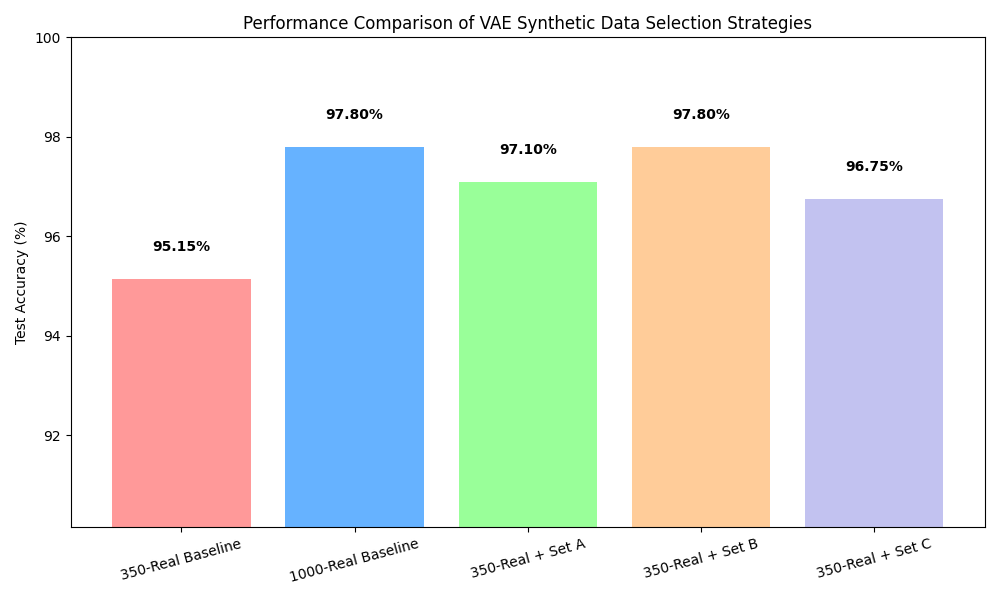
\includegraphics[width=0.85\textwidth]{../Problem_1_VAE/Outputs/5_Evaluation_Plots/vae_benchmarking_results.png}
    \caption{Performance comparison of VAE synthetic data selection strategies.}
    \label{fig:vae_benchmarking}
\end{figure}
